\documentclass{beamer}
\usepackage{ragged2e} %justify text
\usetheme{Madrid}
\usepackage{graphicx}
\usepackage{subfig}
\usepackage{float}
\usepackage{comment}
\setbeamertemplate{enumerate item}{(\alph{enumi})}
\setbeamertemplate{navigation symbols}{}
%Information to be included in the title page:
\title[] %optional
{The network origins of aggregate fluctuations }

%\subtitle{A short story}

\author[] % (optional, for multiple authors)
{D. Acemoglu, V. M. Carvalho, A. Ozdaglar, A. Tahbaz-Salehi  \\
(Econometrica, 2012)}


\date[] % (optional)
{Chris Ackerman \& Antonio Martner\\
Presentation for Econ 241A, UCLA.\\
December 7th, 2021}
\begin{document}

\frame{\titlepage}

%%%%%%%%%%%%%%%%%%%%%%%%%
\begin{frame}
\frametitle{Motivation (1)}
\justifying

{\bf Question:}\\
Do microeconomic sector specific shocks lead to aggregate fluctuations in 
presence of heterogenous intersectoral input–output linkages?\\
\vspace{0.5cm}
{\bf What this paper do:}
\begin{itemize}
  \item Develops a multisector model that captures input–output linkages.
  \item Propose three 3 key theorems to describe how idiosyncratic shocks propagate
  and average out.
  \item Provide an evidence based application of the theory developed.
\end{itemize}

\end{frame}
%%%%%%%%%%%%%%%%%%%%%%%%%
\begin{frame}
    \frametitle{Motivation (2)}
    \justifying
    {\bf Why is this important:}\\
    Independent shocks to specific industries do not vanish as quickly as the
    previous literature proposed, generating more persistent effects that initially
    thought.\\
\vspace{0.5cm}
{\bf Key inside:}\\
Microeconomic shocks effects may not remain confined
to where they originate.\\
$\implies$ Microeconomic shocks may propagate
throughout the economy, affect the output of other sectors, and generate sizable
aggregate effects.\\
\vspace{0.5cm}
    {\bf Main contribution:}\\
    Provide a mathematical
    framework for the analysis of shocks propagations and to characterize
    that their role in aggregate fluctuations depend on the structure of 
    interactions between different sectors.
    
    \end{frame}
%%%%%%%%%%%%%%%%%%%%%%%%%
%\begin{frame}
 %   \frametitle{Table of Contents}
  %  \tableofcontents
%\end{frame}

%%%%%%%%%%%%%%%%%%%%%%%%%


\begin{frame}{Previous argument}
    \justifying
    Idiosyncratic shocks generate that aggregate output concentrates around its mean at a very rapid rate.\\[5pt]
    $\implies$  In an economy consisting of n sectors hit by independent shocks, aggregate fluctuations 
    would have a magnitude proportional to $1/ \sqrt{n}$\\[5pt]
    $\implies$ Negligible effect at
    high levels of disaggregation.\\[10pt]
    
    This argument ignores the presence of interconnections between
    different firms and sectors, functioning as a potential propagation mechanism
    of idiosyncratic shocks throughout the economy.\\
\end{frame}
%%%%%%%%%%%%%%%%%%%%%%%%%


\begin{frame}{Real life statement}
    \justifying
    Ford's CEO requested emergency government support for General Motors and
    Chrysler in nov 2008 (Why in the world he will do that?)\\[10pt]
    
    He argued that, given the significant
    overlap in the suppliers and dealers of the three automakers, the collapse of
    either GM or Chrysler would have a ripple effect across the industry, leading
    to severe disruption of Ford’s production operations within days, if not hours.\\
\end{frame}

%%%%%%%%%%%%%%%%%%%%%%%%%
\begin{frame}{Graph examples: Previous argument works}
    \justifying
   As n increases and the economy becomes more disaggregated,
    the diversification argument based on the LLN
    implies that independent sectoral shocks average out rapidly at the rate
    $\sqrt{n}$.
    
    \begin{figure}[H]
      \caption*{Symmetric economies}
      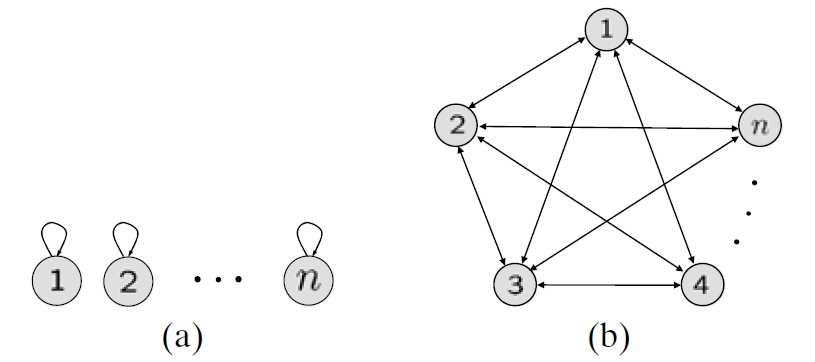
\includegraphics[scale=0.7]{1}
      \centering
    \end{figure}

The symmetric
structure of this economy ensures that aggregate output is a symmetric
function of the shocks to each sector, implying that the diversification argument
remains applicable.

\end{frame}
%%%%%%%%%%%%%%%%%%%%%%%%%
\begin{frame}{Graph examples: Previous argument NOT works}
    \justifying
    Consider  an economy with small number of sectors playing a disproportionately
    important role as input suppliers to others. Consequently, the
    interplay of sectoral shocks and the intersectoral network structure may generate
    sizable aggregate fluctuations.
    
    \begin{figure}[H]
      \caption*{One sector is the only supplier of all other sectors}
      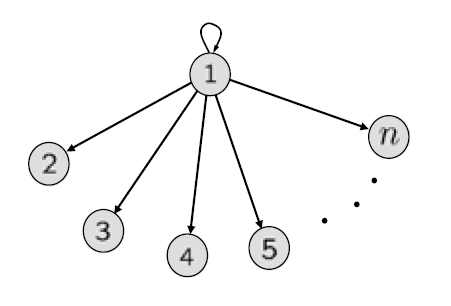
\includegraphics[scale=0.7]{2}
      \centering
    \end{figure}
\end{frame}

%%%%%%%%%%%%%%%%%%%%%%%%%
\begin{frame}{How real graphs look}
    \justifying
    \begin{figure}[H]
        \caption*{Network corresponding to the U.S. input–output matrix in 1997}
        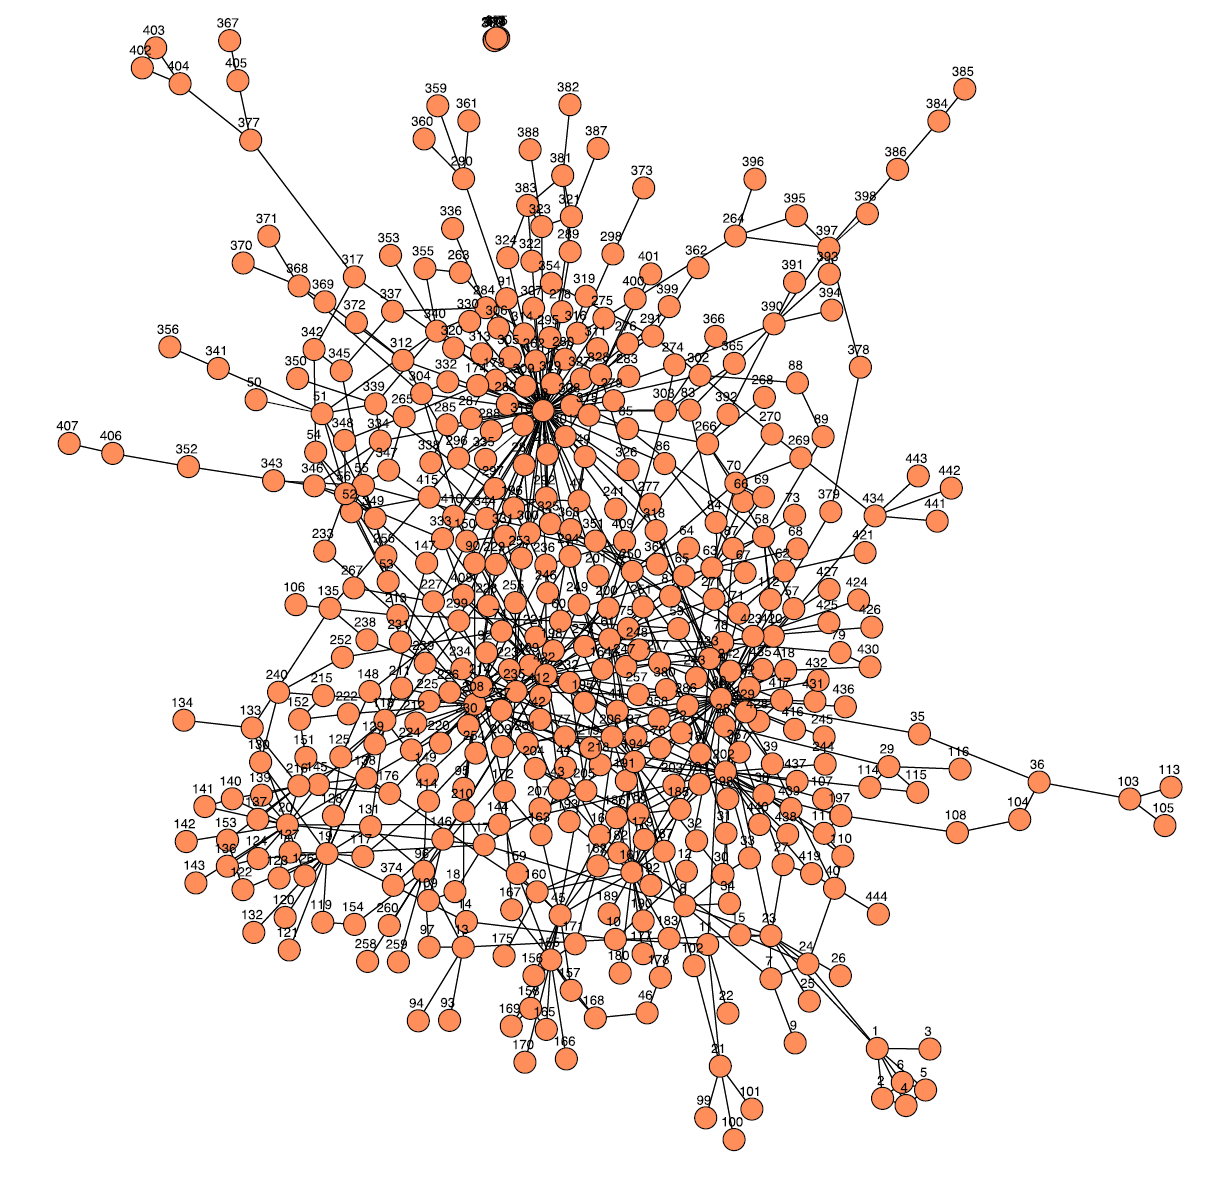
\includegraphics[scale=0.4]{3}
        \centering
      \end{figure}   

      $\implies$  Small number of sectors playing a disproportionately
      important role as input suppliers to others
\end{frame}

%%%%%%%%%%%%%%%%%%%%%%%%%
\begin{frame}{Road map}
    \justifying    

    Investigate whether aggregate volatility, defined as the standard deviation of log
    output, vanishes as $n\rightarrow\infty$.\\[10pt]
    \begin{itemize}
        \justifying    
        \item In certain cases, such as the star network,
        the LLN fails and aggregate output does not concentrate
        around a constant value.
        \item The main focus, however, is on the more interesting cases
        in which the law of large numbers holds, yet the structure of the intersectoral
        network still has a defining effect on aggregate fluctuations.
        \item  Sectoral interconnections may imply that aggregate output concentrates around its
        mean at a rate significantly slower than $\sqrt{n}$.
    \end{itemize} 

    \end{frame}

%%%%%%%%%%%%%%%%%%%%%%%%%
\begin{frame}{Model}
    \justifying
  
\end{frame}

%%%%%%%%%%%%%%%%%%%%%%%%%
\begin{frame}{Theorems}
    \justifying
  
\end{frame}

%%%%%%%%%%%%%%%%%%%%%%%%%
\begin{frame}{Application: Setup}
    \justifying
  {\bf Data:} Detailed
  benchmark input–output accounts spanning the 1972–2002 period, compiled
  every five years by the Bureau of Economic Analysis.\\[5pt]
\begin{figure}[H]
    \caption*{ Intermediate input intensity shares:}
    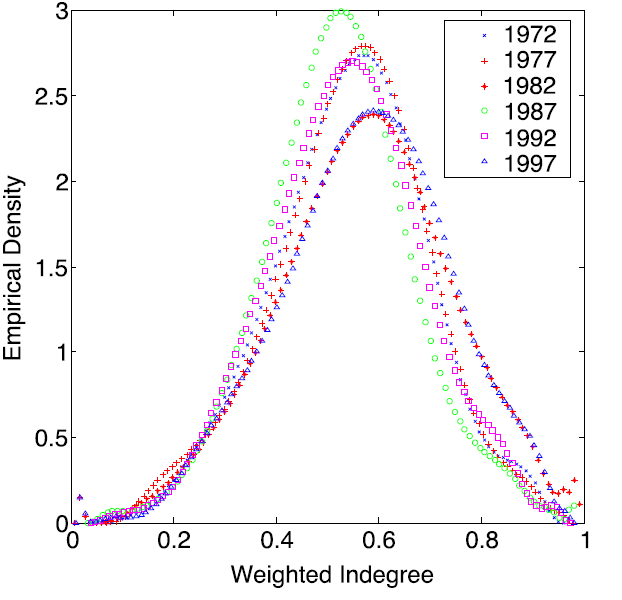
\includegraphics[scale=0.6]{4}
    \centering
\end{figure}   

$\implies$ Most sectors are concentrated around the mean (0.55).: on average, 71\% of the sectors are within one
standard deviation of the mean input share.
\end{frame}

%%%%%%%%%%%%%%%%%%%%%%%%%
\begin{frame}{First- and second-order OUT-degrees densities}
    \justifying
    \begin{figure}[H]
        \caption*{ Intermediate input intensity shares:}
        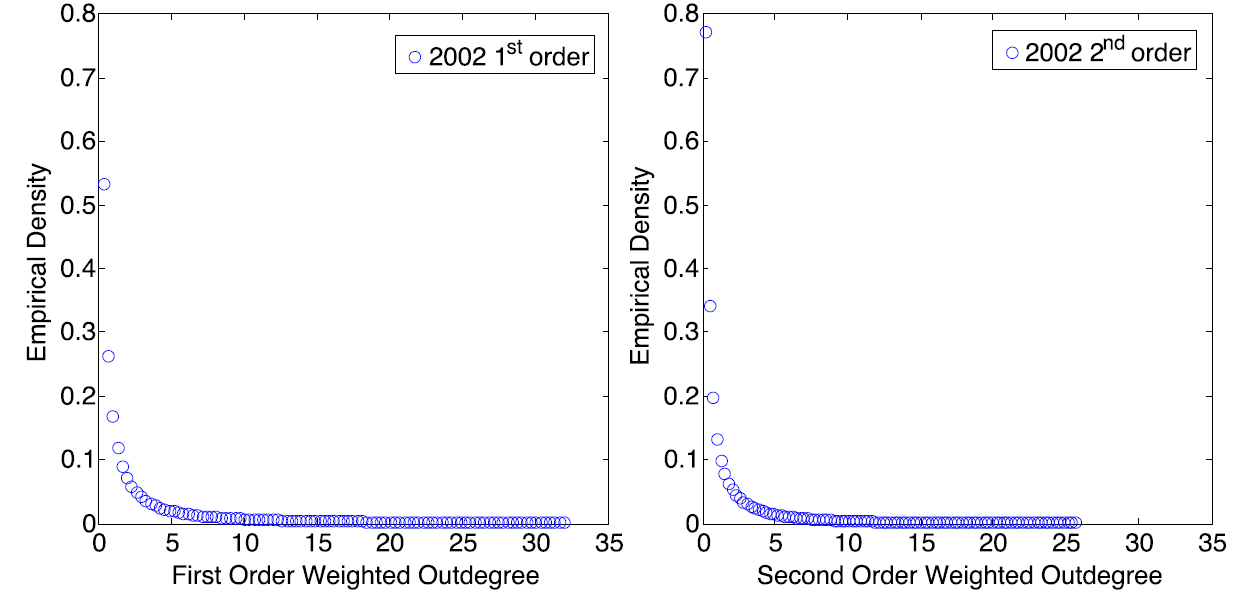
\includegraphics[scale=0.6]{5}
        \centering
    \end{figure}  

Heavy right tails, meaning that some commodities are (1) General purpose inputs used by many other sectors.
and (2) major suppliers to sectors that produce the general purpose inputs.\\[5pt]

$\implies$ The tail of the distributions is well-approximated by a power law
distribution (Pareto distribution).

\end{frame}

%%%%%%%%%%%%%%%%%%%%%%%%%
\begin{frame}{Distribution parameters estimation (1)}
    \justifying
    OLS regression of the empirical log-CCDF
    on the log-outdegree sequence are downward biased in small samples (Gabaix and Ibragimov, 2011).
    Thus implement the modified log rank–
    log size regression. Take 
    the tail of  1 minus the empirical
    cumulative distribution functions to correspond to the top 20\%
    largest sectors in terms of in an out degrees.
    \begin{align*}
        CDF_{\text{Pareto}}=1-\left(\frac{x_m}{x}\right)^\alpha
    \end{align*}
    Where $x_m$ is the scale parameter and $\alpha$ is the shape parameter.
\end{frame}
%%%%%%%%%%%%%%%%%%%%%%%%%
\begin{frame}{Distribution parameters estimation (2)}
    \justifying
    $\hat{\beta}$ and $\hat{\zeta}$ are the shape parameters for the first and 
    second-order degree distribution. (As higher is the shape parameter, more skewed is the distribution.)
    \begin{figure}[H]
        %\caption*{ Intermediate input intensity shares:}
        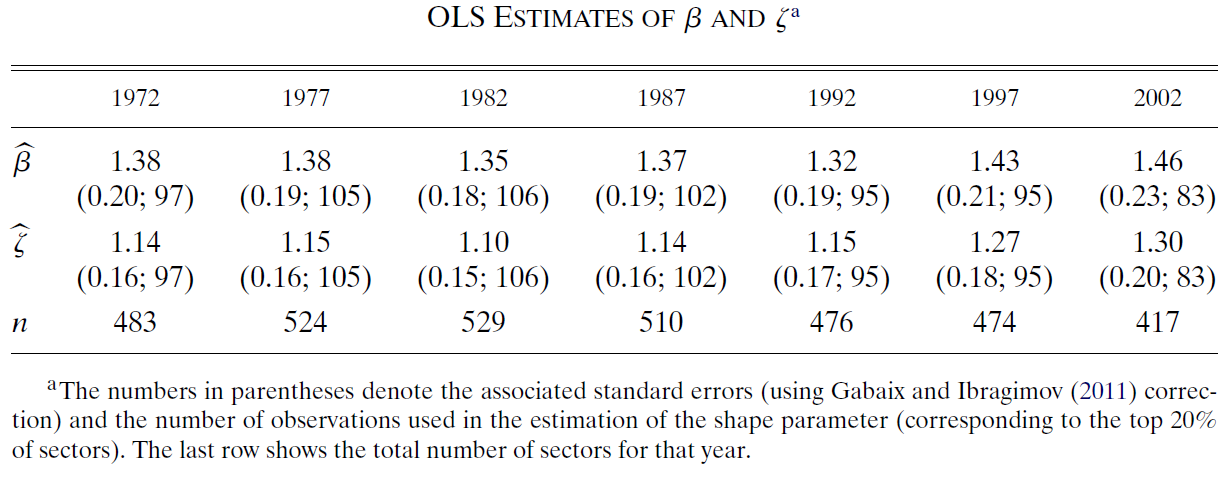
\includegraphics[scale=0.6]{7}
        \centering
\end{figure}  

High degree of asymmetry in the
U.S. economy in terms of the roles that different sectors play as direct or indirect
suppliers to others.\\
$\implies$ The interplay of
sectoral shocks and network effects leads to sizable aggregate fluctuations

\end{frame}
%%%%%%%%%%%%%%%%%%%%%%%%%
\begin{frame}{Quantitative extent of the network effects (1)}
    \justifying
Aggregate effects of sectoral shocks: Compute $||\nu_{n}||_2$
for the U.S. input–output matrix at different levels of 
aggregation and for different years.

\begin{figure}[H]
    %\caption*{ Intermediate input intensity shares:}
    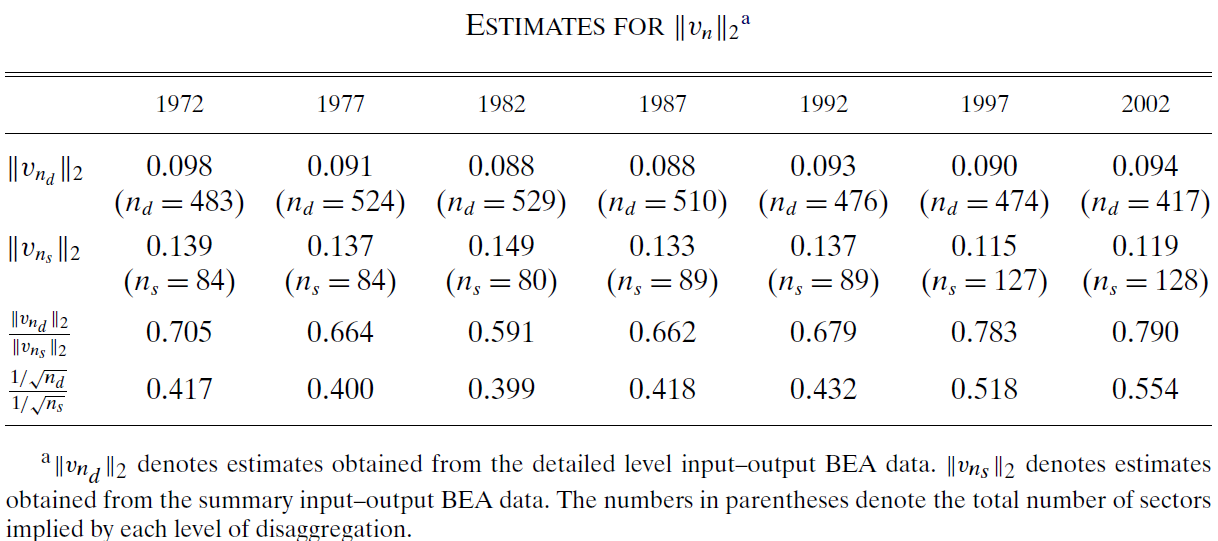
\includegraphics[scale=0.5]{8}
    \centering
\end{figure}  

$||\nu_{n_d}||_2$ at different years
are roughly twice as large as $1/\sqrt{n}$ (First row).\\
$\implies$ intersectoral linkages increase the impact of sectoral 
shocks by at least 2 times.\\[3pt]

The third row captures the change in the aggregate effect of sectoral shocks
from more to less aggregated data.\\
$\implies$ Taking intersectoral linkages into account
simply doubles the impact of sectoral shocks at all levels of disaggregation.
\end{frame}


%%%%%%%%%%%%%%%%%%%%%%%%%
\begin{frame}{Quantitative extent of the network effects (3)}
    \justifying
    If indeed taking intersectoral linkages into account
    simply doubles the impact of sectoral shocks at all levels of disaggregation
    the reatio will be  $\frac{1/\sqrt{n_d}}{1/\sqrt{n_s}}$.\\[5pt]

    If, on the other hand, network effects are more important at higher 
    levels of disaggregation, then we would expect that:
    \begin{align*}
        \frac{||\nu_{n_d}||_2}{||\nu_{n_s}||_2}>\frac{1/\sqrt{n_d}}{1/\sqrt{n_s}}
    \end{align*}


\end{frame}
%%%%%%%%%%%%%%%%%%%%%%%%%
\begin{frame}{Quantitative extent of the network effects (4)}
    \justifying
    The table early shows that the latter is indeed the case for all years. 
    For example, in 1972, as we move
    from the more aggregated measurement at the level of 84 sectors (at two-digit
    SIC) to an economy comprising 483 sectors (roughly at four-digit SIC), the
    standard diversification argument would imply a decline of 58\% in the role of
    sectoral shocks, whereas the actual decline observed in the data (measured by
    $\frac{||\nu_{n_d}||_2}{||\nu_{n_s}||_2}$is about 29\%.
    
\end{frame}

%%%%%%%%%%%%%%%%%%%%%%%%%




%Whereas the lower bound implied by the average shape parameter for the first-order
%degrees, $\beta = 1.38$, is $n(\beta-1)/\beta = n^{0.28}$. It is 
%noteworthy that this is not only a significantly slower rate of decay than
%$\sqrt{n}$ the rate predicted by the standard
%diversification argument.




%%%%%%%%%%%%%%%%%%%%%%%%%
\begin{frame}{Back-of-the-envelope calculation (1)}
    \justifying


    Using TFP estimations across 459 four-digit (SIC) manufacturing industries
    from the NBER productivity database between 1958 and 2005, compute
    its average standard deviation to be 0.058.\\[5pt]

    Average of the U.S. GDP accounted for by manufacturing is around 20\% for the 
    same time frame.\\[5pt]

Assuming that the manufacturing industries 
correspond to one-fifth of the GDP, the economy comprises $5 × 459 = 2295$ 
sectors. With a sector volatility of 0.06, if aggregate volatility decayed at
the rate $\sqrt{n}$, it expects it to be $0.058 / \sqrt{2295}=0.001$.\\[5pt]

\end{frame}

%%%%%%%%%%%%%%%%%%%%%%%%%

\begin{frame}{Back-of-the-envelope calculation (2)}
    \justifying
    The shape parameter for the second order degrees $\hat{\zeta} = 1.18$
    implies that aggregate volatility decays no faster than $n^{(\zeta-1) / \zeta} = n^{0.15}$. \\[10pt]
    
    Using the second-order degree distribution,
    aggregate volatility decays at the rate $n^{0.15}$, the same number would be
    $0.058/2295^{0.15}=0.018$. This corresponds to sizable aggregate fluctuations, in
    the ballpark of the approximately 2\% standard deviation of the U.S. GDP.
\end{frame}
%%%%%%%%%%%%%%%%%%%%%%%%%
\end{document}